\documentclass[journal,12pt,onecolumn]{IEEEtran}
\usepackage{cite}
 \usepackage{caption}
\usepackage{graphicx}
\usepackage{amsmath,amssymb,amsfonts,amsthm}
\usepackage{algorithmic}
\usepackage{graphicx}
\usepackage{textcomp}
\usepackage{xcolor}
\usepackage{txfonts}
\usepackage{listings}
\usepackage{enumitem}
\usepackage{mathtools}
\usepackage{gensymb}
\usepackage{comment}
\usepackage[breaklinks=true]{hyperref}
\usepackage{tkz-euclide} 
\usepackage{listings}
\usepackage{gvv}
%\def\inputGnumericTable{}                                 
\usepackage[latin1]{inputenc} 
\usetikzlibrary{arrows.meta, positioning}
\usepackage{xparse}
\usepackage{color}                                            
\usepackage{array}                                            
\usepackage{longtable}                                       
\usepackage{calc}                                             
\usepackage{multirow}
\usepackage{multicol}
\usepackage{hhline}                                           
\usepackage{ifthen}                                           
\usepackage{lscape}
\usepackage{tabularx}
\usepackage{array}
\usepackage{float}

\usepackage{float}
%\newcommand{\define}{\stackrel{\triangle}{=}}
\theoremstyle{remark}
\usepackage{circuitikz}
\captionsetup{justification=centering}
\usepackage{tikz}

\title{Matrices in Geometry 4.3.24}
\author{EE25BTECH11035 - Kushal B N}
\begin{document}
\vspace{3cm}
\maketitle
{\let\newpage\relax\maketitle}
\textbf{Question: }
Find the ratio in which the line $2x + 3y - 5 = 0$ divides the line segment joining the points $\brak{8,-9}$ and $\brak{2,1}$. Also find the coordinates of the point of division.
\bigskip

\textbf{Given: } \\
Line $\myvec{2 & 3}\myvec{x\\y} = 5$\\
Points $\vec{A}\myvec{8\\-9}$ and $\vec{B}\myvec{2\\1}$
\bigskip

\textbf{Solution: }\\
Let $\vec{P}\myvec{h\\k}$ be the point on the given line dividing the line segment joining the given points. \\
So, the point $\vec{P}$ also lies on the line joining the given points $\vec{A}$ and $\vec{B}$.\\
The direction vector for this line would be\\
\begin{equation}
    \vec{d} = \vec{B} - \vec{A} = \myvec{-6\\10}
\end{equation}

So that the normal vector for the line(after dividing by common factor 2) will be\\
\begin{equation}
    \vec{n} = \myvec{5\\3}
\end{equation}

and in the line equation $\vec{n}^T\vec{P}=c$,\\
\begin{equation}
    c = \myvec{5&3}\myvec{2\\1} = 13
\end{equation}

Thus, the line equation is\\
\begin{equation}
    \myvec{5&3}\myvec{x\\y} = 13
\end{equation}

Solving for the intersection of the two lines, and by forming the augmented matrix,\\
\begin{equation}
    \myvec{2&3\\5&3}\myvec{x\\y} = \myvec{5\\13}
\end{equation}

\begin{equation}
    \implies \myvec{2&3&|&5\\5&3&|&13} \overset{R_1 \rightarrow \frac{1}{2}R_1}{\longrightarrow} \myvec{1&\frac{3}{2}&|&\frac{5}{2}\\5&3&|&13}
\end{equation}

\begin{equation}
    \myvec{1&\frac{3}{2}&|&\frac{5}{2}\\5&3&|&13} \overset{R_2 \rightarrow R_2 - 5R_1}{\longrightarrow} \myvec{1&\frac{3}{2}&|&\frac{5}{2}\\0&\frac{-9}{2}&|&\frac{1}{2}}
\end{equation}

\begin{equation}
    \myvec{1&\frac{3}{2}&|&\frac{5}{2}\\0&\frac{-9}{2}&|&\frac{1}{2}} \overset{R_2 \rightarrow \frac{-2}{9}R_2}{\longrightarrow} \myvec{1&\frac{3}{2}&|&\frac{5}{2}\\0&1&|&\frac{-1}{9}} 
\end{equation}

\begin{equation}
    \implies \vec{P} = \myvec{\frac{8}{3}\\ \frac{-1}{9}}
\end{equation}

Section Formula for a point $\vec{P}$ which divides the line segment formed by points $\vec{A}$ and $\vec{B}$ in the ratio $k:1$ is given by\\
\begin{equation}
    \vec{P} = \frac{k\vec{B}+\vec{A}}{k+1}
\end{equation}

\begin{equation}
    k\brak{\vec{P}-\vec{B}} = \vec{A} - \vec{P}
\end{equation}

\begin{equation}
    \implies k = \frac{\brak{\vec{A}-\vec{P}}^{\top}\brak{\vec{P}-\vec{B}}}{\norm{\vec{P}-\vec{B}}^2}
\end{equation}

\begin{equation}
    \brak{{\vec{A}-\vec{P}}}^{\top}\brak{\vec{P}-\vec{B}} = \myvec{\frac{16}{3}&\frac{-80}{9}}\myvec{\frac{2}{3}\\ \frac{-10}{9}} = \frac{1088}{81}
\end{equation}

\begin{equation}
    {\norm{\vec{P}-\vec{B}}}^2 = \brak{\vec{P}-\vec{B}}^{\top}\brak{\vec{P}-\vec{B}} = \frac{136}{81}
\end{equation}

\begin{equation}
    \implies \fbox{k=8}
\end{equation}

\textbf{Final Answer: }\\
$\therefore$ The ratio in which the line divides the two given points is 8:1 and the coordinates of the point of division is $\myvec{\frac{8}{3}\\ \frac{-1}{9}}$.

\begin{figure}[H]
    \centering
    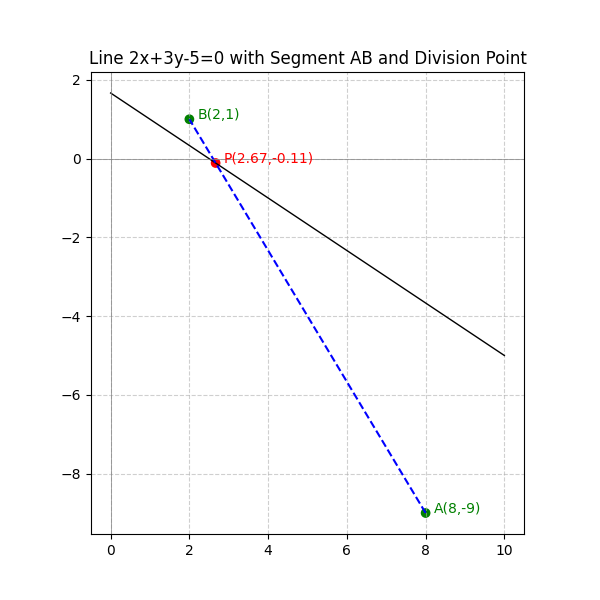
\includegraphics[width=0.72\columnwidth]{figs/2.png}
    \caption{}
    \label{fig:placeholder}
\end{figure}
\end{document}